\documentclass[preview]{standalone}
\usepackage{tikz}
\usetikzlibrary{decorations.pathmorphing, shapes.geometric}

\RequirePackage{amsmath,amsfonts,amssymb}
% Definición de colores personalizados
\definecolor{primaryColor}{RGB}{20,45,105} % color primario
\definecolor{secondaryColor}{RGB}{0,100,160} % Color secundario

\begin{document}
            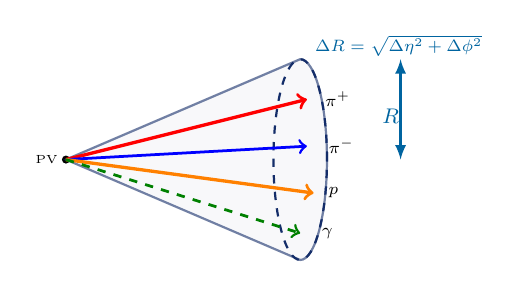
\begin{tikzpicture}[scale=0.85, transform shape]
                % Vértice de colisión
                \fill[black] (0,0) circle (0.06);
                \node[left] at (0,0) {\tiny PV};
                
                % Cono de Apertura del Jet (3D usando elipses)
                \draw[thick, primaryColor, fill=primaryColor!5, opacity=0.6] (0,0) -- (3.5,1.5) arc (90:-90:0.4cm and 1.5cm) -- cycle;
                \draw[thick, primaryColor, dashed] (3.5,0) ellipse (0.4cm and 1.5cm);
                
                % Partículas estables reales dentro del cono
                \draw[line width=1.2pt, ->, red] (0,0) -- (3.6,0.9);
                \node[right, black] at (3.75,0.9) {\scriptsize $\pi^+$};
                
                \draw[line width=1pt, ->, blue] (0,0) -- (3.6,0.2);
                \node[right, black] at (3.8,0.2) {\scriptsize $\pi^-$};
                
                \draw[line width=1.2pt, ->, orange] (0,0) -- (3.7,-0.5);
                \node[right, black] at (3.8,-0.5) {\scriptsize $p$};
                
                \draw[line width=1pt, ->, green!50!black, dashed] (0,0) -- (3.5,-1.1);
                \node[right, black] at (3.7,-1.1) {\scriptsize $\gamma$};
                
                % Indicador del Radio del Cono (Delta R)
                \draw[latex-latex, secondaryColor, thick] (5,0) -- (5,1.5);
                \node[left, secondaryColor] at (5.1,0.65) {\small $R$};
                \node[right, secondaryColor] at (3.6,1.7) {\scriptsize $\Delta R = \sqrt{\Delta\eta^2 + \Delta\phi^2}$};
            \end{tikzpicture}
\end{document}